
\documentclass[10pt]{beamer} 
%\usetheme{Warsaw}
\usetheme{CambridgeUS}


\usepackage{graphicx,hyperref,url}
\usepackage[utf8]{inputenc}
\usepackage[T1]{fontenc}
\usepackage[portuges,brazilian]{babel}
%%%\usepackage{wrapfig}
\usepackage{caption}
\usepackage{subfigure}
%\usepackage{subcaption}
\usepackage{latexsym}
\usepackage{amssymb, amsmath}
\usepackage{multicol}
\usepackage{pifont}%,bbding}%%,dingbat} %%% ver manual de simbolos
\usepackage[final]{listings}
\usepackage{comment}


\definecolor{azulclaro}{rgb}{0.9,0.9,0.9}
\definecolor{mygreen}{rgb}{0,0.6,0}
\definecolor{mygray}{rgb}{0.5,0.5,0.5}
\definecolor{mymauve}{rgb}{0.58,0,0.82}
\definecolor{darkgray}{rgb}{.4,.4,.4}
\definecolor{purple}{rgb}{0.65, 0.12, 0.82}

\newcommand{\minizinc}{MiniZinc}

\lstset{ 
  %  label={pgm_ex01},
    backgroundcolor=\color{azulclaro}, 
    language=erlang, %%Miranda,%%Perl,%%%Python, %%Mercury,
    showstringspaces=false,
    basicstyle=\bf\scriptsize\ttfamily,
%%      basicstyle= \footnotesize %%% TESTAR
%%      keywordstyle=\bfseries\color{green!40!black},
    keywordstyle=\textbf{\color{mygreen}}, 
    otherkeywords={*, \%, array, constraint, solve, output,  show, "/\", satisfy, set, of, if, then, elseif, float, search},
%%  keywordstyle=\color{blue},       % keyword style
%%    commentstyle=\itshape\color{purple!40!black},
      commentstyle=\color{orange},    % comment style
      identifierstyle=\color{blue},
      stringstyle=\color{orange},
      stringstyle=\color{mymauve},
      numbers=left,  % where to put the line-numbers; possible values are (none, left, right)
      numbersep=5pt,   % how far the line-numbers are from the code
      numberstyle=\tiny\color{magenta},
      keepspaces=true      
    % %caption={LEGENDA no source PASCAL ficou OK},
}


\graphicspath{{/home/ccs/Dropbox/figs_genericas/}{figuras/}{/home/ccs/Dropbox/CCS/picat}}
\DeclareGraphicsExtensions{.pdf,.png,.jpg}
%Global Background must be put in preamble
%\usebackgroundtemplate{\includegraphics[width=\paperwidth]{amarelinho.pdf}}
%%% \begin{frame}[allowframebreaks=0.8]

% The log drawn in the upper right corner.

%\logo{\centering
%\includegraphics[height=0.050\paperheight]{figuras/logo_SBPO_Peixe.png}
%%\hspace{9.6cm}
%\includegraphics[height=0.027\paperheight]{figuras/logo_udesc_horizontal.jpg}


%%%%%%%%%%%%%%%%%%%%%%%%%%%%%%%%%%%%%%%%%%%%%%%%%%%%%%%%%%%%%%%%%%%%%


\title[Picat]{\fontsize{20}{30}\selectfont \textcolor{black}{Resumindo e Conectando a Teoria da Complexidade Computacional em Figuras}}

\author[]{Claudio Cesar de Sá\\
     {\small \url{claudio.sa@udesc.br}}}

\institute[UDESC]{
    Departamento de Ci\^encia da Computa\c{c}\~ao \\
    Centro de Ci\^encias e Tecnol\'ogias\\
   Universidade do Estado de Santa Catarina}

%%%%%%%%%%%%%%%%%%%%%%%%%%%%%%%%%%%%%%%%%%%%%%%%%%%%%%%%%%%%%%%%%%%%%

\begin{document}

\begin{frame}
    \titlepage
\end{frame}

%%%%%%%%%%%%%%%%%%%%%%%%%%%%%%%%%%%%%%%%%%%%%%%%%%%%%%%%%%%%%%%%%%%%%

%\begin{frame} [allowframebreaks=0.8]
%\frametitle{Sumário}
%\tableofcontents
%\end{frame}

%%%%%%%%%%%%%%%%%%%%%%%%%%%%%%%%%%%%%%%%%%%%%%%%%%%%%%%%%%%%%%%%%%%%%

\begin{frame}[fragile]

\frametitle{Contextualizando}

\begin{itemize}
	\item As figuras vieram de vários autores \textit{by Google}
	\item Cabeçalhos e sequência -- do autor
	\item Requisitos: Finalizando um curso de LFA ou de TEC
\end{itemize}

\end{frame}



%-----------------------------------------------------------------------------
\begin{frame}[fragile]

\frametitle{Resolvendo Problemas}

\begin{figure}[!ht]
	\centering
	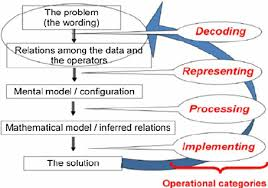
\includegraphics[height =.65\textheight,width=.7\textwidth]
	{figuras/ciclo_problema_solucao.jpeg}
	\caption{O  quê o cientista busca?}
	%\label{ag_01}
\end{figure}



\end{frame}
%-----------------------------------------------------------------------------



%-----------------------------------------------------------------------------
\begin{frame}[fragile]

\frametitle{O Dilema dos Problemas  é:}

\begin{figure}[!ht]
\centering

\includegraphics[height =.65\textheight,width=.8\textwidth]
{figuras/dilema_eh.jpg}
%%%\caption{Agente situado versus a visão clássica de sistemas inteligentes}
%\label{ag_01}
\end{figure}

\end{frame}
%-----------------------------------------------------------------------------







%-----------------------------------------------------------------------------
\begin{frame}[fragile]

\frametitle{Os  Problemas -- Tipos}
\begin{figure}[!ht]
\centering
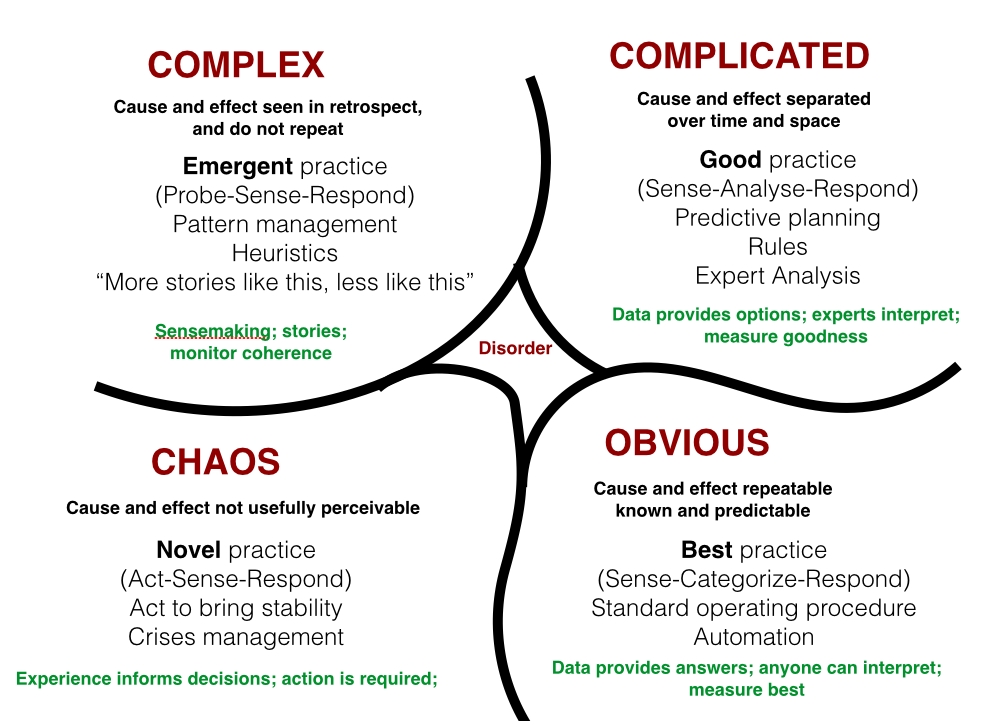
\includegraphics[height =.65\textheight,width=.8\textwidth]
{figuras/os_problemas.png}
\caption{A área de algoritmos se preocupa com os  dificeis (complicados) e os simples (os ingênuos)}
%\label{ag_01}
\end{figure}

\end{frame}


%-----------------------------------------------------------------------------
\begin{frame}[fragile]

\frametitle{A área da CC se preocupa com:}
\begin{figure}[!ht]
	\centering
	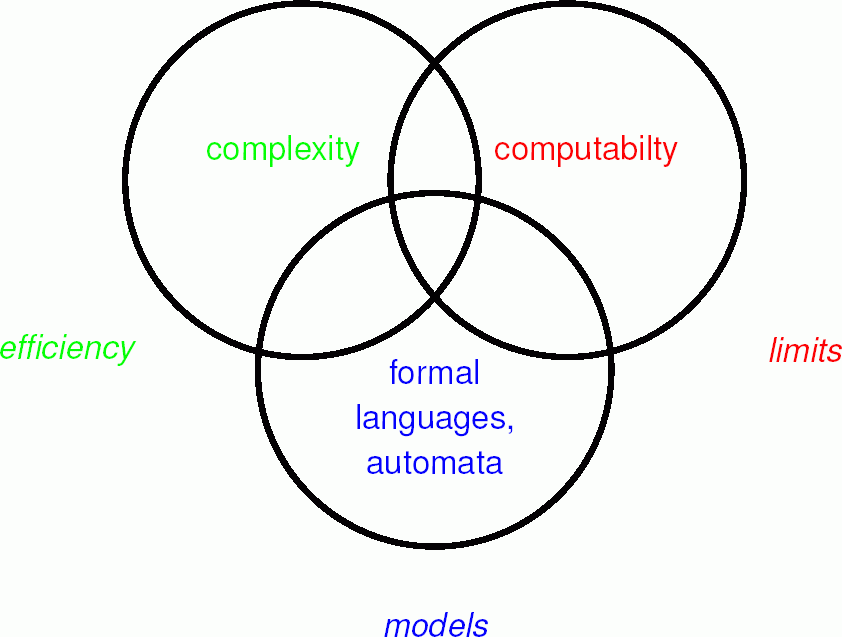
\includegraphics[height =.65\textheight,width=.8\textwidth]
	{figuras/modelos_complexidade_computabilidade.png}
	\caption{Precisamos construir modelos e medir seu desempenho}
	%\label{ag_01}
\end{figure}

\end{frame}


%-----------------------------------------------------------------------------




%-----------------------------------------------------------------------------
\begin{frame}[fragile]

\frametitle{A área da CC se preocupa com:}
\begin{figure}[!ht]
	\centering
	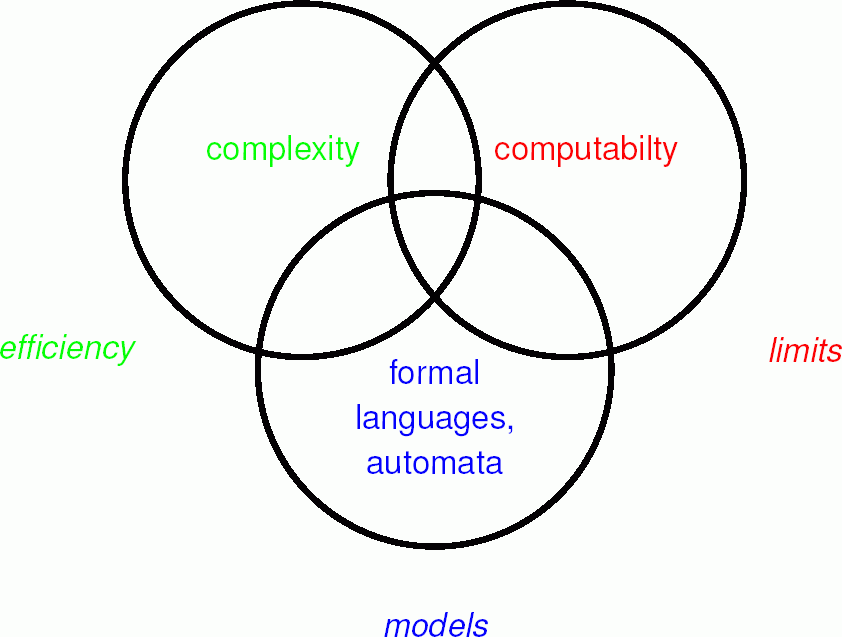
\includegraphics[height =.65\textheight,width=.8\textwidth]
	{figuras/modelos_complexidade_computabilidade.png}
	\caption{Precisamos construir modelos e medir seu desempenho}
	%\label{ag_01}
\end{figure}

\end{frame}


%-----------------------------------------------------------------------------
\begin{frame}[fragile]
\frametitle{Um escopo de formalismos para CC:}
\begin{figure}[!ht]
	\centering
	\includegraphics[height =.6\textheight,width=.9\textwidth]
%	{figuras/theoretical_computer_science.pdf}
		{figuras/theoretical_computer_science02.pdf}
	%\caption{A área de algoritmos se preocupa com os  dificeis (complicados) e os simples (os ingênuos)}
	%\label{ag_01}
\end{figure}

\end{frame}




%-----------------------------------------------------------------------------










%-----------------------------------------------------------------------------







\begin{frame}[fragile]
\frametitle{LFA -- Linguagens  Formais}
\begin{figure}[!ht]
	\centering
	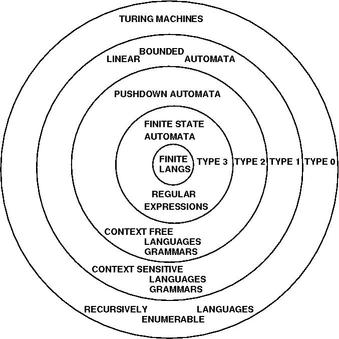
\includegraphics[height =.5\textheight,width=.5\textwidth]
	{figuras/Chomsky_Venn.jpg}
	%\caption{}
	%\label{ag_01}
\end{figure}

\end{frame}




%-----------------------------------------------------------------------------

\begin{frame}[fragile]

%\frametitle{Precisamos Mensurar esta Complexidade -- Dificuldade}
\frametitle{Uma máquina \textit{ forte }e robusta: Máquina de Turing}
\begin{figure}[!ht]
\centering
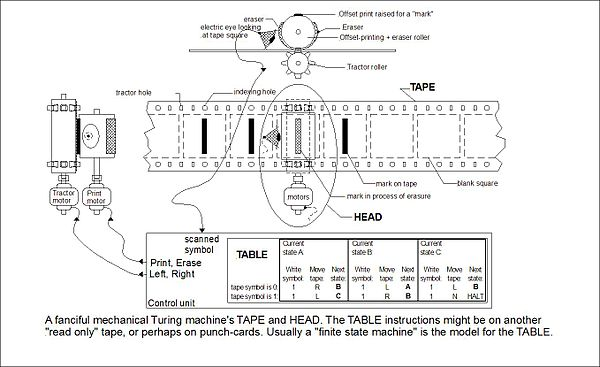
\includegraphics[height =.65\textheight,width=.8\textwidth]
{figuras/turing_machine_mecanica.jpg}
%%\caption{$\Sigma = \{1,2\}$ -- Partida $\models w = 11221 ... 12 $}
%\label{ag_01}
\end{figure}

\end{frame}



%-----------------------------------------------------------------------------


%-----------------------------------------------------------------------------
\begin{frame}[fragile]

\frametitle{Especificamente interessa a área de algoritmos:}

\begin{figure}[!ht]
\centering
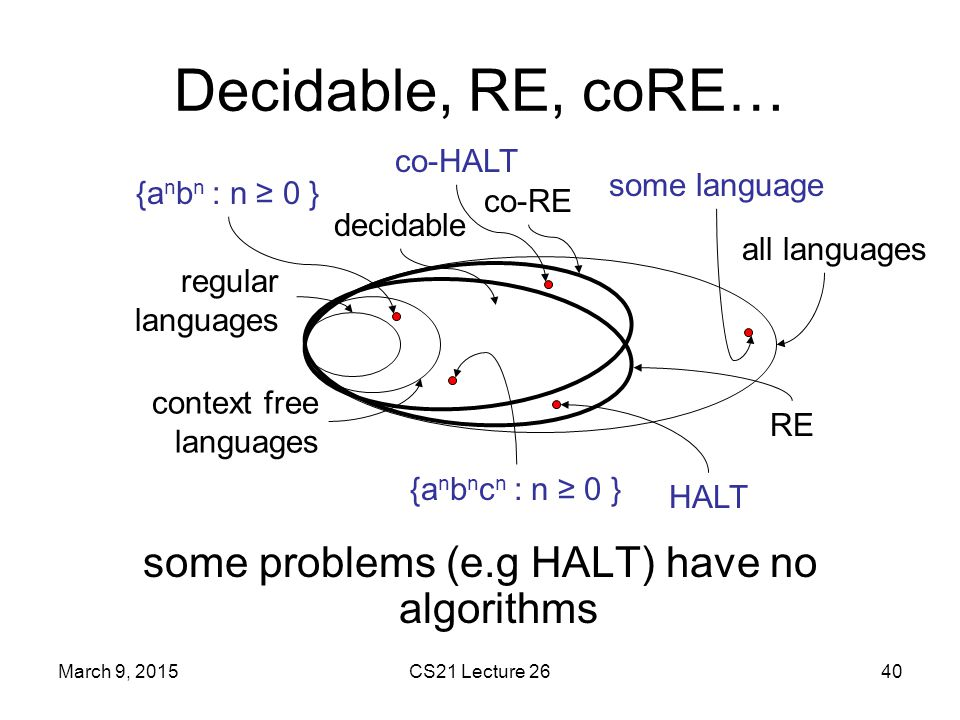
\includegraphics[height =.65\textheight,width=.8\textwidth]
{figuras/some+problems+have+no+algorithms_HALT.jpg}
\caption{RE: reconhecíveis $\approx $ linguagens finitas ou não, mas sem garantias
da existência de um algortimo que \textbf{SEMPRE} pare!}
%\label{ag_01}
\end{figure}

\end{frame}





%-----------------------------------------------------------------------------
\begin{frame}[fragile]

\frametitle{Ampliando a visão anterior tem-se: linguagens, máquinas -- modelos abstratas  versus problemas resolvidos (total -- parcial) }

\begin{figure}[!ht]
\centering
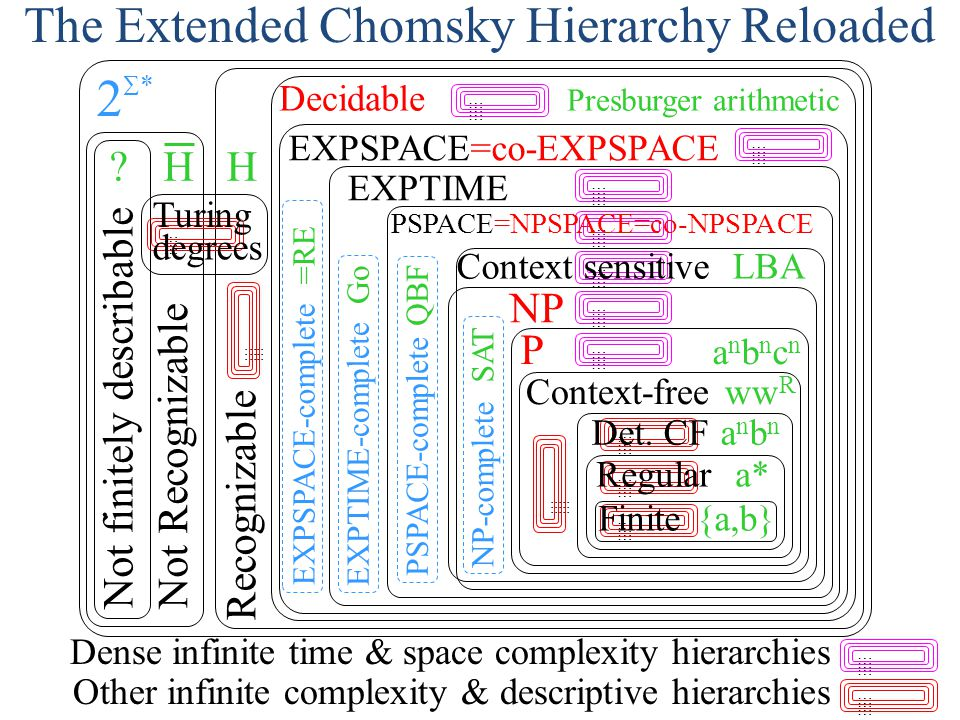
\includegraphics[height =.65\textheight,width=.8\textwidth]
{figuras/Extended+Chomsky+Hierarchy.jpg}
\caption{Modelos, formalismos, máquinas e complexidade!}
%\label{ag_01}
\end{figure}

\end{frame}
%-----------------------------------------------------------------------------


\begin{frame}[fragile]
\frametitle{Em geral, o cientista de CC está focado em questões de:}
\begin{figure}[!ht]
	\centering
	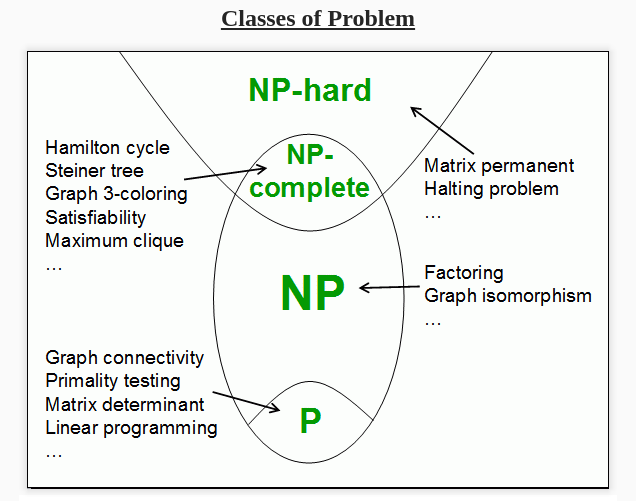
\includegraphics[height =.7\textheight,width=.8\textwidth]
	{figuras/classes_de_problemas.png}
	%\caption{}
	%\label{ag_01}
\end{figure}

\end{frame}

%%%%%%%%%%%%%%%%%%%%%%%%%%%%%%%%%%%%%%%%%%%%%%%%%%%%%%%%%%%%%%%%%%%%%


\begin{frame}[fragile]
\frametitle{Conclusões}
\begin{itemize}
	\item 
		\item 
			\item 
\end{itemize}

\end{frame}



\end{document}
